\subsection{\newrevision{Scheduled-Node Energy, Test Results and Optional Solar Supply}}
\label{sec:estimated_power_budget}
\begingroup\color{green!45!black}
The team reports test results of 5.7 J per active wake-up and approximately 0.77 Wh/day at the battery side. These replace the earlier planning totals as the prototype results. Battery runtime is calculated from the daily consumption, not measured in a full discharge test. The test instrument, traces and repetitions have not yet been documented. The energy analysis uses the agreed schedule: eight hourly measurements from 22:00 to 06:00, and four measurements at four-hour intervals from 06:00 to 22:00. Wake-ups occur at 22:00, 23:00, 00:00--05:00, then 06:00, 10:00, 14:00 and 18:00: twelve per day without double-counting the boundaries. Each sensing ESP32 acquires a signal, performs local inference, forwards its result and returns to sleep. The estimate covers one sensing node; the continuously listening head and server require separate power budgets. The active-stage breakdown and custom-board/solar comparisons below remain estimates.

\paragraph{Assumed active stages}
Table~\ref{tab:assumed_active_stages} retains the earlier 20 s stage budget for comparison with the 5.7 J test result. Individual stage durations and energies have not been reported separately. The 20 s active duration remains an assumption. The 33, 42 and 53 mA observations in Table~\ref{tab:mode_current} are used as approximate whole-node current proxies at a common nominal 5 V; they are not new 5 V measurements. The sensing observation was made at 4.8 V. Communication is assigned a separate 100 mA whole-node allowance for radio operation, beacon waiting and acknowledgments. It is an assumption, not the isolated 3.3 V radio measurement, and is not added to another ESP32 baseline.

\begin{table}[htbp]
\centering\small\color{green!45!black}
\caption{\newrevision{Earlier assumed stages and the newly reported total active energy.}}
\label{tab:assumed_active_stages}
\begin{tabular}{lrrr}
\toprule
Stage & Time (s) & Current (mA) & Energy (J) \\
\midrule
Wake and setup & 3 & 33 & 0.495 \\
Signal acquisition & 10 & 42 & 2.100 \\
Preprocessing and inference & 2 & 53 & 0.530 \\
LoRa result delivery and ACK & 5 & 100 & 2.500 \\
\midrule
Assumed-stage total & 20 & --- & 5.625 \\
Team-reported active test & --- & --- & 5.700 \\
\bottomrule
\end{tabular}
\end{table}
\FloatBarrier

For cycle accounting, the reported 5.7 J is treated as node-input active energy; its test measurement boundary should be confirmed. Using $E=VIt$, the reported 4 mA sleep reading is treated as the complete sleeping load at the nominal 5 V node input. Any connected loads not included in that reading would increase the estimate. The hourly cycle contains 20 s active and 3,580 s asleep; the four-hour cycle contains 20 s active and 14,380 s asleep. Active time is included in each interval, rather than added after it:
\[
E_{\mathrm{hour}}=5.7+0.020(3{,}580)=77.3\ \mathrm{J},
\]
\[
E_{\mathrm{four\ hours}}=5.7+0.020(14{,}380)=293.3\ \mathrm{J}.
\]
The daily total is
\[
E_{5\mathrm{V}}=\frac{8(77.3)+4(293.3)}{3{,}600}
=0.4977\ \mathrm{Wh/day}.
\]
The node is awake for 240 s and asleep for 86,160 s per day. Sleep contributes 0.4787 Wh, approximately 96\% of the 5 V energy budget; the active stages contribute 0.0190 Wh. Average current at this boundary is approximately 4.15 mA.

\paragraph{Battery-side demand and autonomy}
The conversion model assumes an 85\% load-conversion factor and separately reserves 2 mA of standing consumption at the nominal 3.7 V battery for otherwise unmeasured upstream circuitry. Neither value is measured. The 85\% factor excludes this separately budgeted standing drain, avoiding double-counting:
\[
E_{\mathrm{battery,model}}=\frac{E_{5\mathrm{V}}}{0.85}
 +3.7(0.002)(24)=0.7631\ \mathrm{Wh/day}.
\]
The model gives approximately 0.763 Wh/day, close to the team's approximately 0.77 Wh/day test result. The reported 0.77 Wh/day is used for prototype autonomy and solar balance below; the assumed conversion model is retained for sensitivity and custom-board comparisons.

For one nominal 3.7 V, 2,600 mAh battery, nameplate energy is 9.62 Wh. Retaining the assumed 80\% usable fraction gives 7.696 Wh:
\[
T_{\mathrm{prototype}}=\frac{3.7(2.6)(0.80)}{0.77}
\approx\mathbf{10.0\ days}.
\]
This calculated runtime uses the team-reported daily demand. It is not an observed discharge duration; actual usable capacity, cutoff, temperature and ageing affect the result.

\begin{table}[htbp]
\centering\small\color{green!45!black}
\caption{\newrevision{Sensitivity to assumed battery-side standing consumption; 85\% load conversion and 80\% usable battery energy retained.}}
\label{tab:power_overhead_sensitivity}
\begin{tabular}{rrr}
\toprule
Standing drain (mA) & Battery demand (Wh/day) & No-solar autonomy (days) \\
\midrule
0 & 0.585 & 13.1 \\
2 (model allowance) & 0.763 & 10.1 \\
5 & 1.029 & 7.5 \\
\bottomrule
\end{tabular}
\end{table}
\FloatBarrier

As a retry stress case, allocating 120 s rather than 5 s to communication at every wake-up raises battery demand to approximately 0.980 Wh/day and reduces no-solar autonomy to 7.9 days, retaining the other working assumptions. Actual processing, admission and retry times should replace these allowances after integrated tests.

\paragraph{Estimated custom board without development-board overhead}
A custom implementation can omit the development board's USB-to-UART circuitry and use suitable low-power 3.3 V regulation. The ESP32 datasheet gives 10~$\mu$A for the chip with RTC timer and RTC memory retained \cite{espressif_esp32_datasheet}; the complete node also includes sensor, radio and regulator loads. Therefore, 10~$\mu$A is not assigned as a measured whole-node current.

To isolate the sleep-current effect, the comparison retains the prototype's 5.7 J active-energy budget, twelve wake-ups, 20 s assumed active duration, 85\% load-conversion factor, 2 mA battery-side standing allowance and 80\% usable battery energy. The custom sleeping load is supplied at 3.3 V, not the development board's 5 V input. For assumed total sleeping current $I_c$ in amperes,
\[
E_{\mathrm{custom}}=
\frac{0.0190+3.3I_c(86{,}160/3{,}600)}{0.85}
+3.7(0.002)(24).
\]
The retained conversion factor is a comparison assumption, not a specified custom-regulator efficiency. Active energy may also change after redesign, but no such saving is assumed here.

\begin{table}[htbp]
\centering\small\color{green!45!black}
\caption{\newrevision{Prototype result and estimated custom-board cases. All runtimes use 7.696 Wh usable battery energy and exclude solar.}}
\label{tab:custom_board_energy}
\begin{tabular}{p{0.41\linewidth}rrr}
\toprule
Case & Sleep load & Wh/day & Days \\
\midrule
Development-board prototype & 4 mA at 5 V & 0.770 & 10.0 \\
Custom node, assumed & 1 mA at 3.3 V & 0.293 & 26.3 \\
Custom node, assumed & 0.1 mA at 3.3 V & 0.209 & 36.8 \\
Chip-only sleep limit & 10 $\mu$A at 3.3 V & 0.201 & 38.3 \\
\bottomrule
\end{tabular}
\end{table}
\FloatBarrier

The illustrative 0.1--1 mA complete-node cases give approximately \textbf{26--37 days without solar}. These are scenario estimates, not measured custom-board performance. Achieving these currents may require sensor-conditioning power gating and radio shutdown between measurements, as well as low-power regulation; removing the USB-to-UART circuitry alone does not establish them. The 38.3-day chip-only case is an optimistic reference that assumes negligible peripheral sleep draw, while still retaining the upstream 2 mA allowance. That allowance alone consumes 0.1776 Wh/day; removing development-board overhead does not remove it automatically.

\begin{figure}[htbp]
\centering
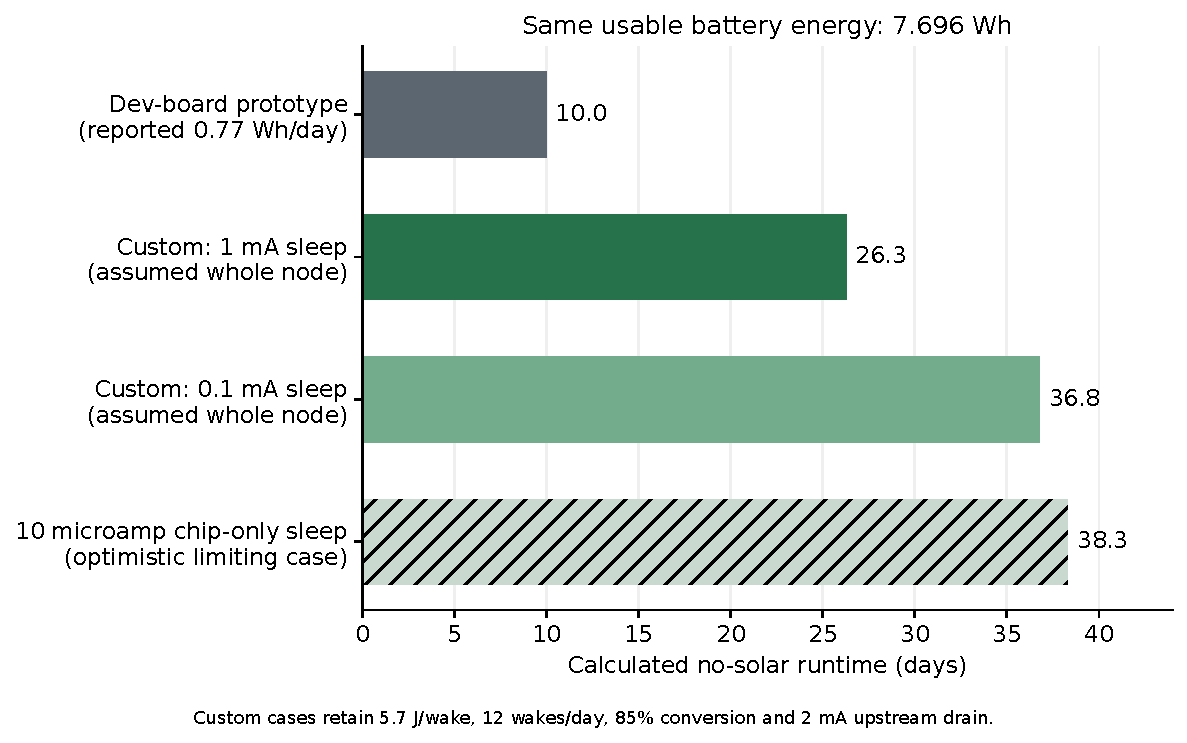
\includegraphics[width=0.95\linewidth]{figures/custom_board_power_comparison.pdf}
\caption{\newrevision{Calculated no-solar runtime from the reported prototype daily demand and explicit custom-board scenarios. Custom active energy and upstream standing drain are held constant; chip-only sleep is an optimistic limit.}}
\label{fig:custom_board_power_comparison}
\end{figure}
\FloatBarrier

\paragraph{Optional 1 W panel}
Panel rating is peak power, not energy available continuously. Daily energy can be estimated from rated power, equivalent peak-sun-hours and a loss factor; temperature, dirt and shading affect output \cite{franklin2019solar}. Here, 2, 4 and 6 peak-sun-hours are scenario assumptions, not measured Sharjah irradiance. A combined factor of 60\% is assumed from nameplate-equivalent generation to usable battery-side energy, covering panel derating, wiring and charging losses. It is a planning allowance, not the published grid-system derate factor in the reference. No grid inverter is included:
\[
E_{\mathrm{solar}}=(1\ \mathrm{W})H(0.60).
\]

\begin{table}[htbp]
\centering\small\color{green!45!black}
\caption{\newrevision{Potential daily energy from a 1 W panel under assumed sunlight and 60\% overall harvest efficiency. Net balance uses the team-reported 0.77 Wh/day prototype demand.}}
\label{tab:solar_energy_estimate}
\begin{tabular}{rrr}
\toprule
Peak-sun-hours & Harvest (Wh/day) & Net balance (Wh/day) \\
\midrule
0 & 0.00 & $-0.77$ \\
2 & 1.20 & $+0.43$ \\
4 (working estimate) & 2.40 & $+1.63$ \\
6 & 3.60 & $+2.83$ \\
\bottomrule
\end{tabular}
\end{table}
\FloatBarrier

At four peak-sun-hours, potential harvest is about 3.1 times the reported prototype battery demand. Break-even is approximately 1.28 peak-sun-hours/day with the assumed losses, or a 0.32 W panel at four peak-sun-hours. Thus a \textbf{1 W panel is a plausible candidate for one scheduled sensing node} under these assumptions. The battery bridges darkness and low-output periods; excess harvest is curtailed when charging or storage limits are reached. This energy balance does not establish year-round autonomy or power for the head.

\begin{figure}[htbp]
\centering
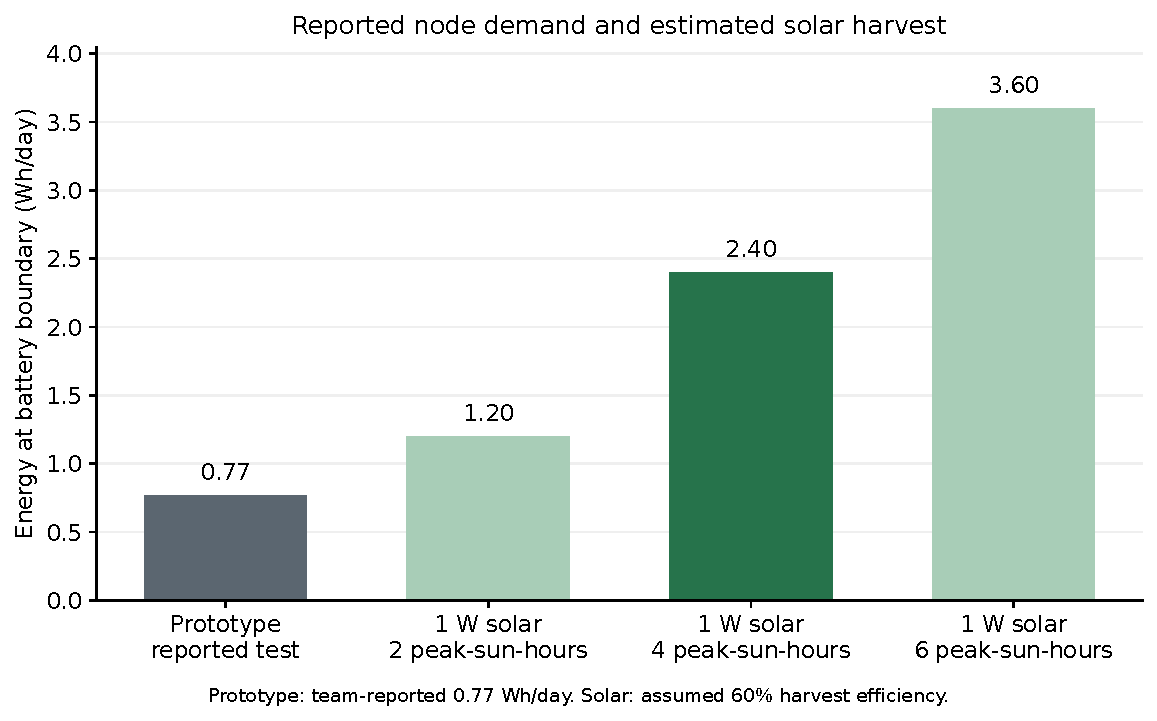
\includegraphics[width=0.95\linewidth]{figures/estimated_node_solar_energy.pdf}
\caption{\newrevision{Team-reported prototype battery demand compared with potential solar harvest. Solar outputs remain estimates using the stated sunlight and harvest-efficiency assumptions.}}
\label{fig:estimated_node_solar_energy}
\end{figure}
\FloatBarrier

Solar hardware remains unpurchased and untested. A suitable panel voltage, charge-current setting and charging/power-path arrangement must be checked with the battery and load; the existing USB-powered TP4056 setup does not demonstrate operation from a variable, current-limited panel. For scale, 1 W at a nominal 5 V is only 200 mA before losses. Installation should give the panel an unshaded exposure rather than place it behind the trunk or foliage. Final validation will log complete-cycle battery energy and daily harvested energy at the intended site.
\endgroup
\FloatBarrier
